%META {"question":"Trên hình có năm tia chung gốc O, không có cặp tia nào đối nhau. Có tất cả bao nhiêu góc (không kể góc bẹt)?","options":["10 góc","8 góc","5 góc","15 góc"],"answer":0,"note":"Mỗi cặp tia tạo đúng một góc: chọn 2 trong 5 tia được 5 × 4 : 2 = 10 góc."}
\documentclass[border=5pt]{standalone}
\usepackage{tkz-euclide}
% Màu dùng chung cho toàn bộ hình vẽ (ảnh stack với nền tối của web)
\definecolor{tminc}{RGB}{226,232,240}   % chữ + nét chính
\definecolor{tmblue}{RGB}{0,210,255}    % nhấn neon xanh
\definecolor{tmpink}{RGB}{255,0,200}    % nhấn neon hồng
\definecolor{tmgreen}{RGB}{0,255,136}   % nhấn neon xanh lá
\color{tminc}

\begin{document}
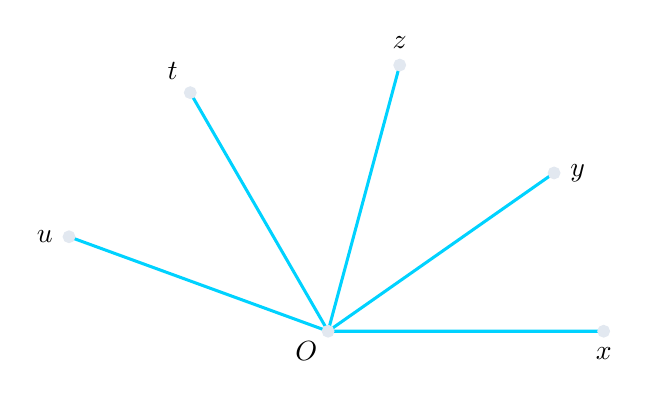
\begin{tikzpicture}[line width=1.1pt]
  \coordinate (O) at (0,0);
  \coordinate (A) at (3.5,0);
  \coordinate (B) at (2.87,2.01);
  \coordinate (C) at (0.91,3.38);
  \coordinate (D) at (-1.75,3.03);
  \coordinate (E) at (-3.29,1.2);
  \draw[tmblue] (O) -- (A) (O) -- (B) (O) -- (C) (O) -- (D) (O) -- (E);
  \tkzDrawPoints[size=3.5,color=tminc,fill=tminc](O,A,B,C,D,E)
  \tkzLabelPoint[below left](O){$O$}
  \tkzLabelPoint[below=2pt](A){$x$}
  \tkzLabelPoint[right=2pt](B){$y$}
  \tkzLabelPoint[above=2pt](C){$z$}
  \tkzLabelPoint[above left=1pt](D){$t$}
  \tkzLabelPoint[left=2pt](E){$u$}
\end{tikzpicture}
\end{document}
